\documentclass[../lecture4-functions.tex]{subfiles}

\begin{document}

\section{Function Header and Body}

% -------------------------------------------------------------------

\begin{frame}[fragile]{Header}
    The function is defined below the body of \mintinline{cpp}{int main()}. The \textbf{header} in this example:

    \begin{cppcode}[lastline = 1, fontsize=\footnotesize]
int factorial(int number);
    \end{cppcode}

    indicates that the \verb|factorial()| function expects to be \textbf{passed} an integer value (the parameter type) from the main body of the program and that the value passed will be stored locally in a variable named \verb|number| (the formal parameter name). \newline

    The \verb|return value type| of the function is also \verb|int| in this example, indicating that at the end of executing the body of the function, an integer value will be returned to the statement in which the function was called. Functions which do not return a value have \verb|return value type| void.
\end{frame}

% -------------------------------------------------------------------

\begin{frame}[fragile]{Body}
    The \textbf{body} of the funcction computes the factorial of a number in exactly the same way as in the example with only a \mintinline{cpp}{main()} function. \newline

    The execution of the function terminates with a \verb|return statement|:

    \begin{cppcode}[lastline = 1, fontsize=\footnotesize]
        return factorial;
    \end{cppcode}

    which specifies that the value stored in the function variable factorial should be passed back to the calling function.
\end{frame}

% -------------------------------------------------------------------

\begin{frame}[fragile]{xkcd Programming Memes}
    \begin{center}
        \makebox[\textwidth]{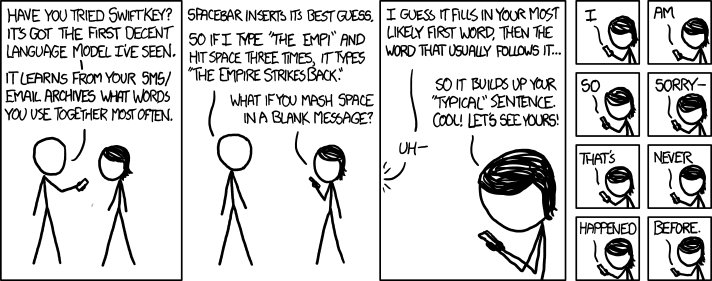
\includegraphics[width=0.90\paperwidth,height=0.90\textheight]{graphics/xkcd-swiftkey.png}}
    \end{center}
\end{frame}

% -------------------------------------------------------------------

\end{document}
